\section{Anexo}

\subsection{Colecciones y Carga de Datos}
\begin{figure}[H]
    \centering
    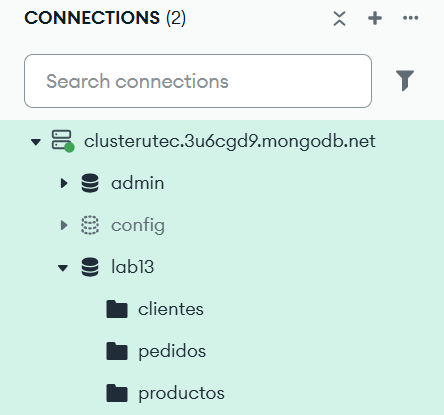
\includegraphics[width=0.4\textwidth]{./p1_collections.png}
    \caption{Colecciones creadas en MongoDB}\label{fig:collections}
\end{figure}

\begin{figure}[H]
    \centering
    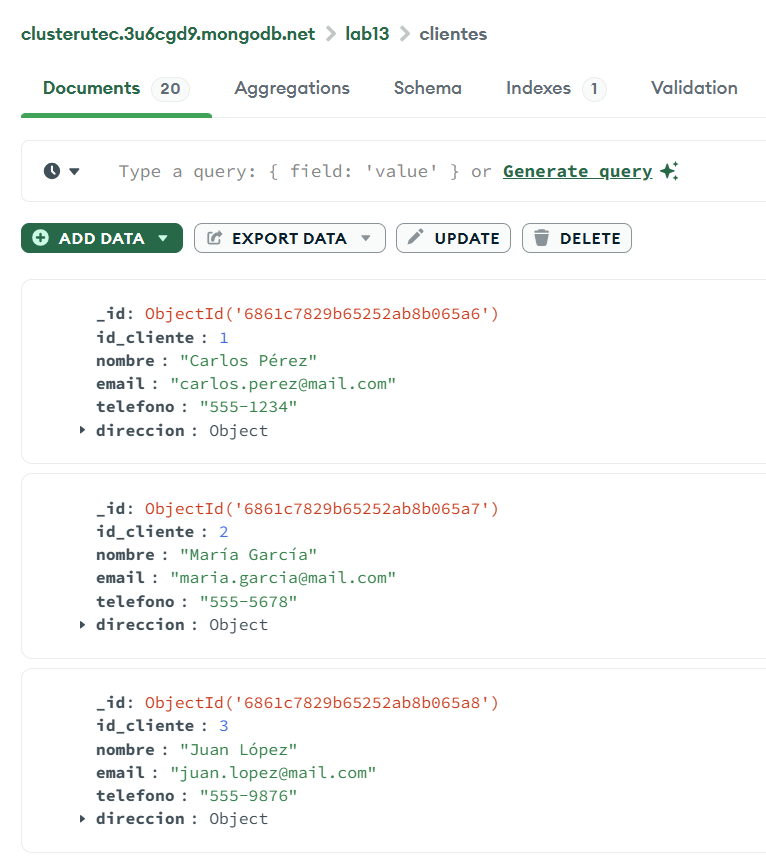
\includegraphics[width=0.7\textwidth]{./p1_clientes.png}
    \caption{Clientes en MongoDB Compass}\label{fig:clientes}
\end{figure}

\newpage
\subsection{Consultas}\label{consultas}

\begin{figure}[H]
    \centering
    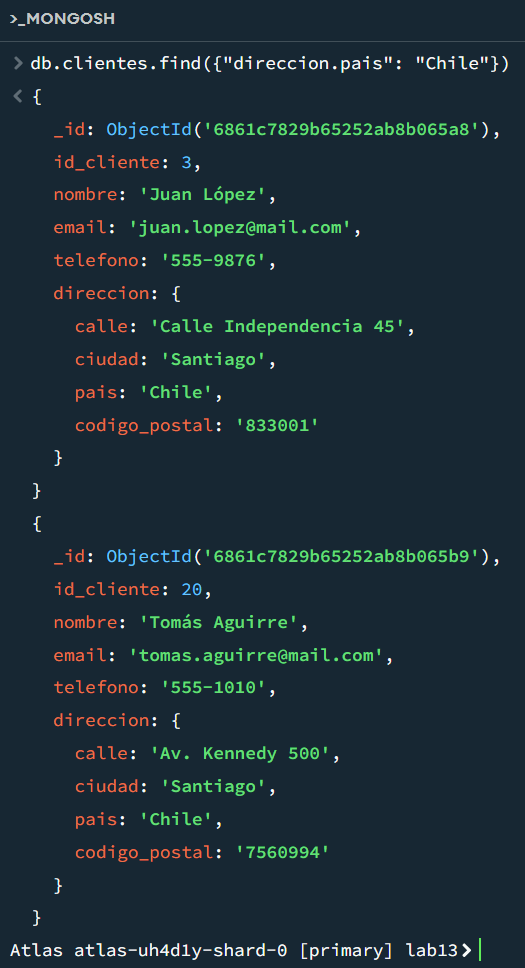
\includegraphics[width=0.6\textwidth]{./p1_chile.png}
    \caption{Obtener todos los clientes de Chile}\label{fig:chile}
\end{figure}

\begin{figure}[H]
    \centering
    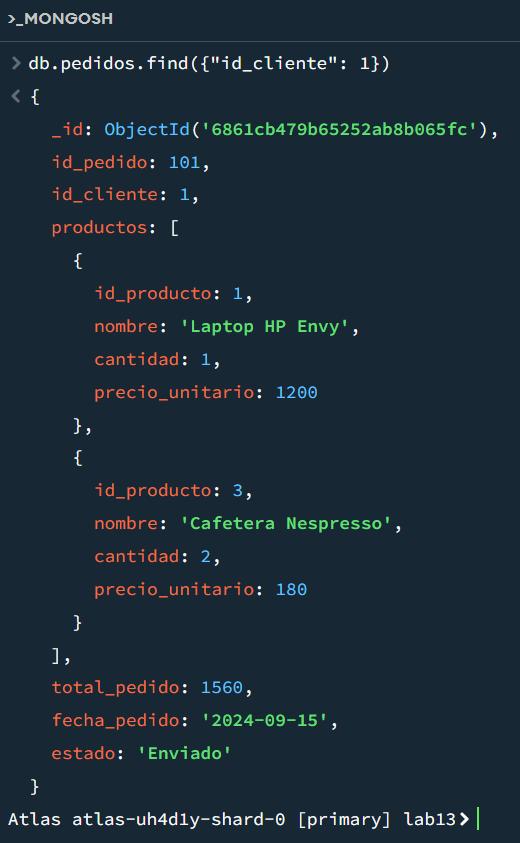
\includegraphics[width=0.6\textwidth]{./p1_id.png}
    \caption{Obtener los pedidos de un cliente específico (por ID)}\label{fig:id}
\end{figure}

\begin{figure}[H]
    \centering
    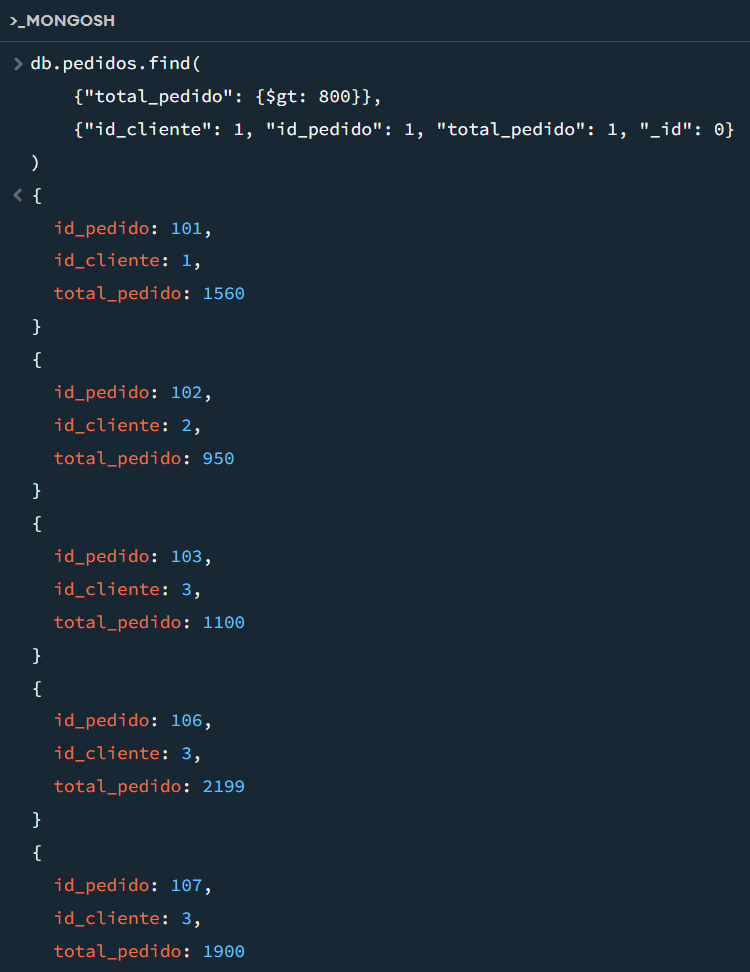
\includegraphics[width=0.6\textwidth]{./p1_superior.png}
    \caption{Obtener los pedidos con un total superior a cierto valor}\label{fig:superior}
\end{figure}

\begin{figure}[H]
    \centering
    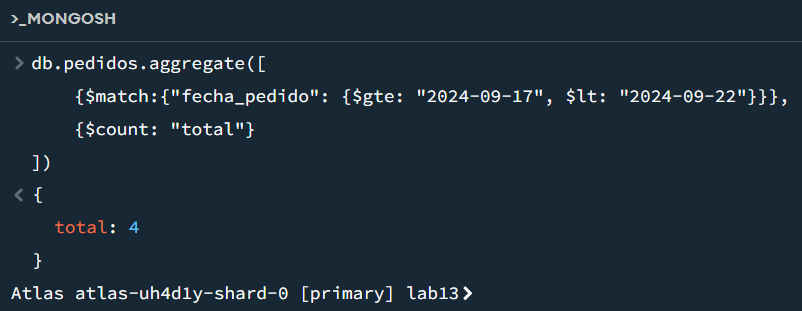
\includegraphics[width=0.6\textwidth]{./p1_rangofecha.png}
    \caption{Obtener los pedidos en un rango de fechas}\label{fig:rangofecha}
\end{figure}

\begin{figure}[H]
    \centering
    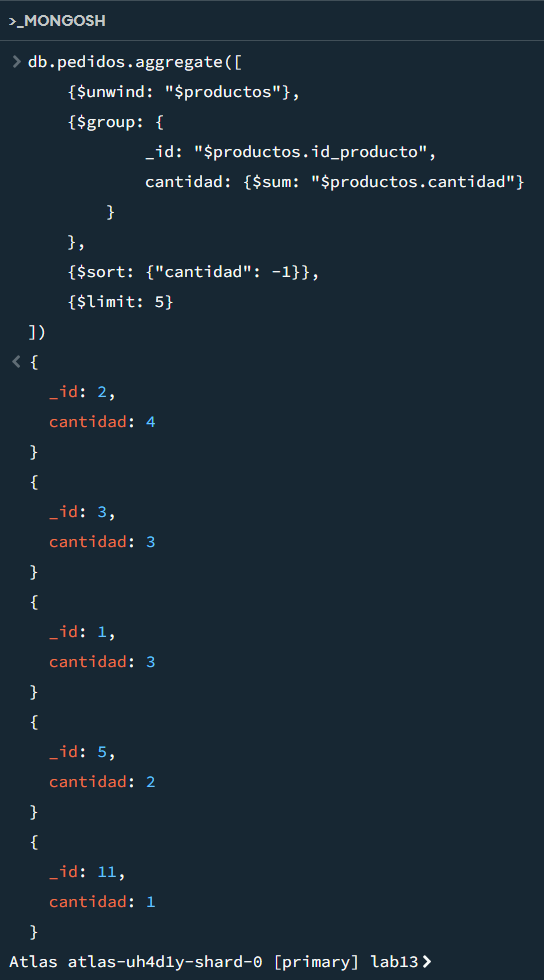
\includegraphics[width=0.6\textwidth]{./p1_kmasvendidos.png}
    \caption{Obtener los $k$ productos más vendidos}\label{fig:kmasvendidos}
\end{figure}

\begin{figure}[H]
    \centering
    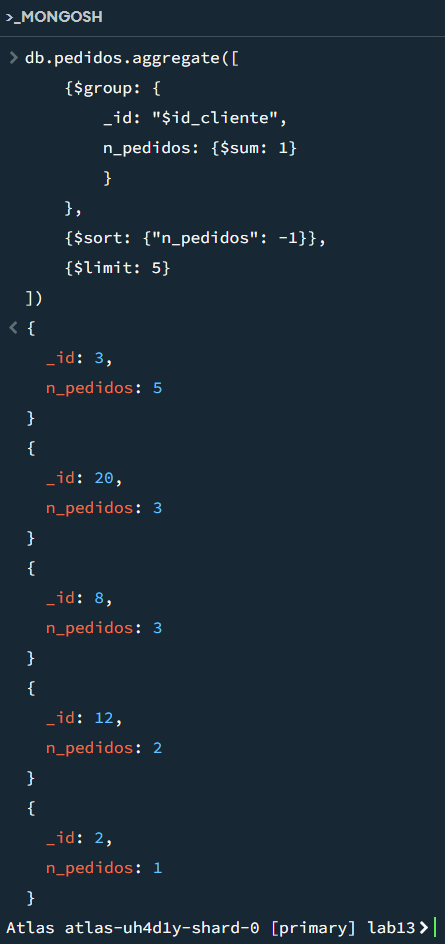
\includegraphics[width=0.6\textwidth]{./p1_kmasfrecuentes.png}
    \caption{Obtener los clientes más frecuentes}\label{fig:kmasfrecuentes}
\end{figure}

\begin{figure}[H]
    \centering
    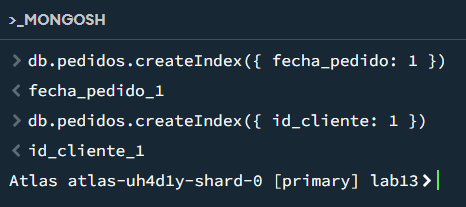
\includegraphics[width=0.6\textwidth]{./p1_creacionindices.png}
    \caption{Creación de índices en MongoDB Compass}\label{fig:creacionindices}
\end{figure}

\subsection{Índices}
\begin{figure}[H]
    \centering
    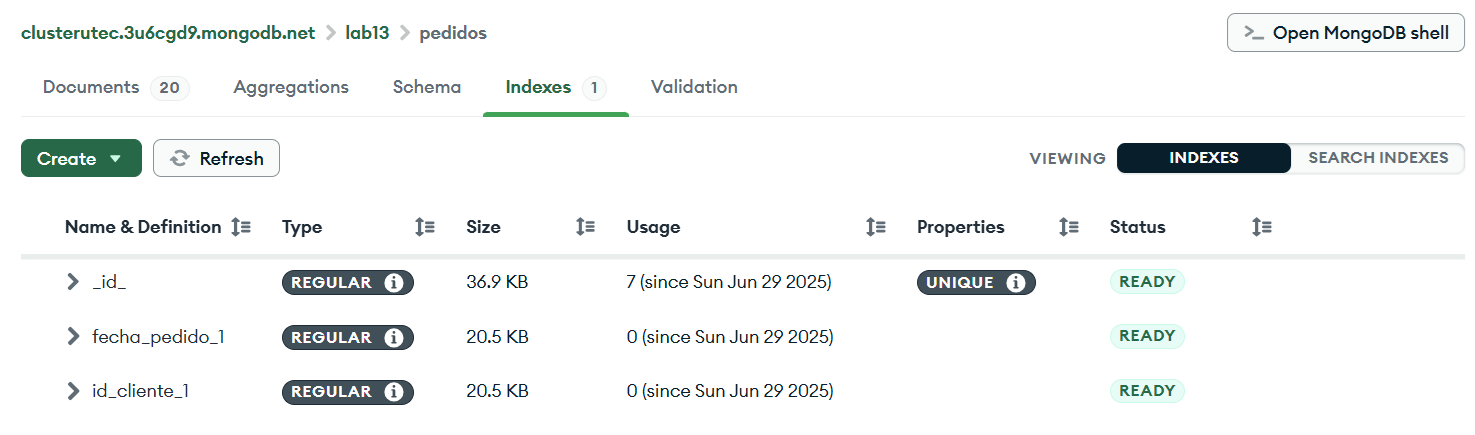
\includegraphics[width=1\textwidth]{./p1_indices.png}
    \caption{Índices creados en MongoDB Compass}\label{fig:indices}
\end{figure}

\subsection{Carga de Datos con Python}\label{cargadatos}

\begin{figure}[H]
    \centering
    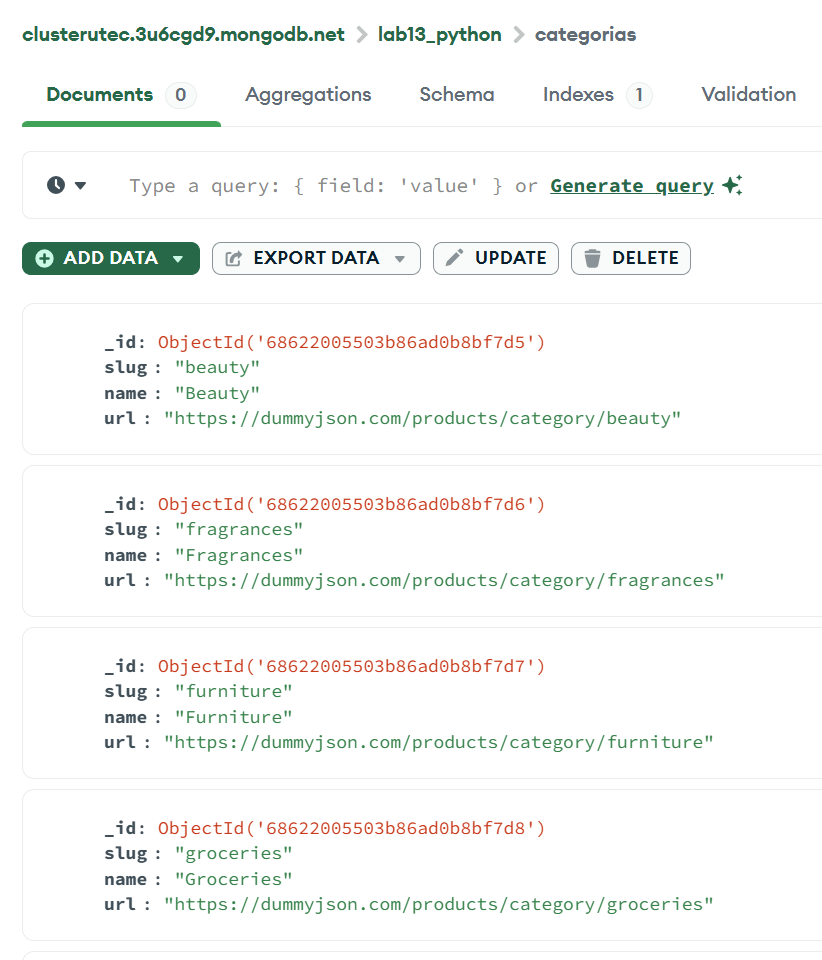
\includegraphics[width=0.6\textwidth]{./p2_categorias.png}
    \caption{Categorías cargadas en MongoDB desde Python}\label{fig:pythoncategorias}
\end{figure}

\begin{figure}[H]
    \centering
    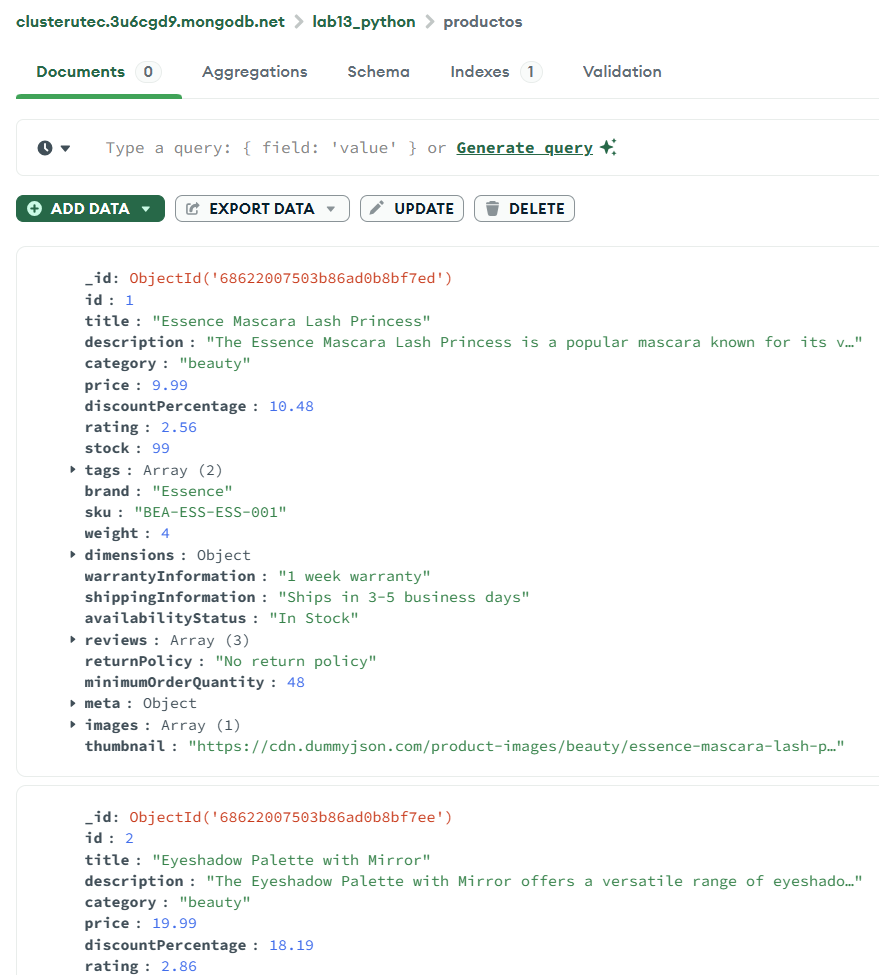
\includegraphics[width=0.6\textwidth]{./p2_productos.png}
    \caption{Productos cargados en MongoDB desde Python}\label{fig:pythonproductos}
\end{figure}

\subsection{Implementación MongoDBHandler}\label{repo}

$\bullet$ Enlace al repositorio: \url{https://github.com/Jvnc0503/BD2-Labs/tree/main/Lab13/lab13.ipynb}